\documentclass[uplatex,dvipdfmx,a4paper,10pt]{jsarticle}

\usepackage{amsmath,amsthm,amssymb}
\usepackage[dvipdfmx]{graphicx}
\usepackage{bm}
\usepackage{ascmac}
%
\usepackage{multirow}
\usepackage{wrapfig}

\usepackage{xcolor}

\usepackage{textcomp}
%
\pagestyle{empty}
%% 高さの設定
\usepackage{geometry}
\geometry{left=25truemm, right=25truemm, top=25truemm, bottom=25truemm}

%
\abovecaptionskip=-1pt
%\belowcaptionskip=-1pt
%
\renewcommand{\baselinestretch}{0.9} % 全体の行間調整
\renewcommand{\figurename}{Fig.}
\renewcommand{\tablename}{Tab.}
%
\makeatletter 
\def\section{\@startsection {section}{1}{\z@}{1.5 ex plus 2ex minus -.2ex}{0.5 ex plus .2ex}{\large\bf}}
\def\subsection{\@startsection{subsection}{2}{\z@}{0.2\Cvs \@plus.5\Cdp \@minus.2\Cdp}{0.1\Cvs \@plus.3\Cdp}{\reset@font\normalsize\bfseries}}
\makeatother 
%
\graphicspath{{../../fig/}}
%
\title{ポリカーボネートの力学特性評価 I\\~ポリカーボネートの降伏挙動の追試~}
% \subtitle{ポリカーボネートの降伏挙動とエンタルピー緩和}
\author{東亞合成 佐々木裕}
\date{\today}

\begin{document}

\maketitle

\section{やりたいこと}

\begin{description}
	\item[大目標] 
	接着剤の主成分である高分子材料のバルクでの力学特性を、とくに破壊挙動に注目して整理したい。
	\item[中目標] 
	高分子の特徴的な2つの状態について評価
	\begin{itemize}
		\item ガラス状態での破壊挙動について
		\begin{itemize}
			\item ポリカーボネート(以下、PC)を対象として
			\item ネットワークポリマーであるエポキシ樹脂を対象として
		\end{itemize}
		\item ゴム状態での破壊挙動
		\begin{itemize}
			\item 詳細については今後策定
		\end{itemize}
	\end{itemize}
	\item[小目表] 
	PCのガラス状態について評価
	\color{red}
	\begin{itemize}
		\item PCの降伏挙動の変形速度依存性の追試(本ドキュメント)
		\color{black}
		\item PCの降伏挙動とエンタルピー緩和との関係について(上記に基づき検討予定)
		\item 上記関係と破壊挙動との相関を明らかに(連続して実施予定)
	\end{itemize}
\end{description}

\begin{wrapfigure}{r}{0.5\textwidth} %% 図右寄せの場合{r}
	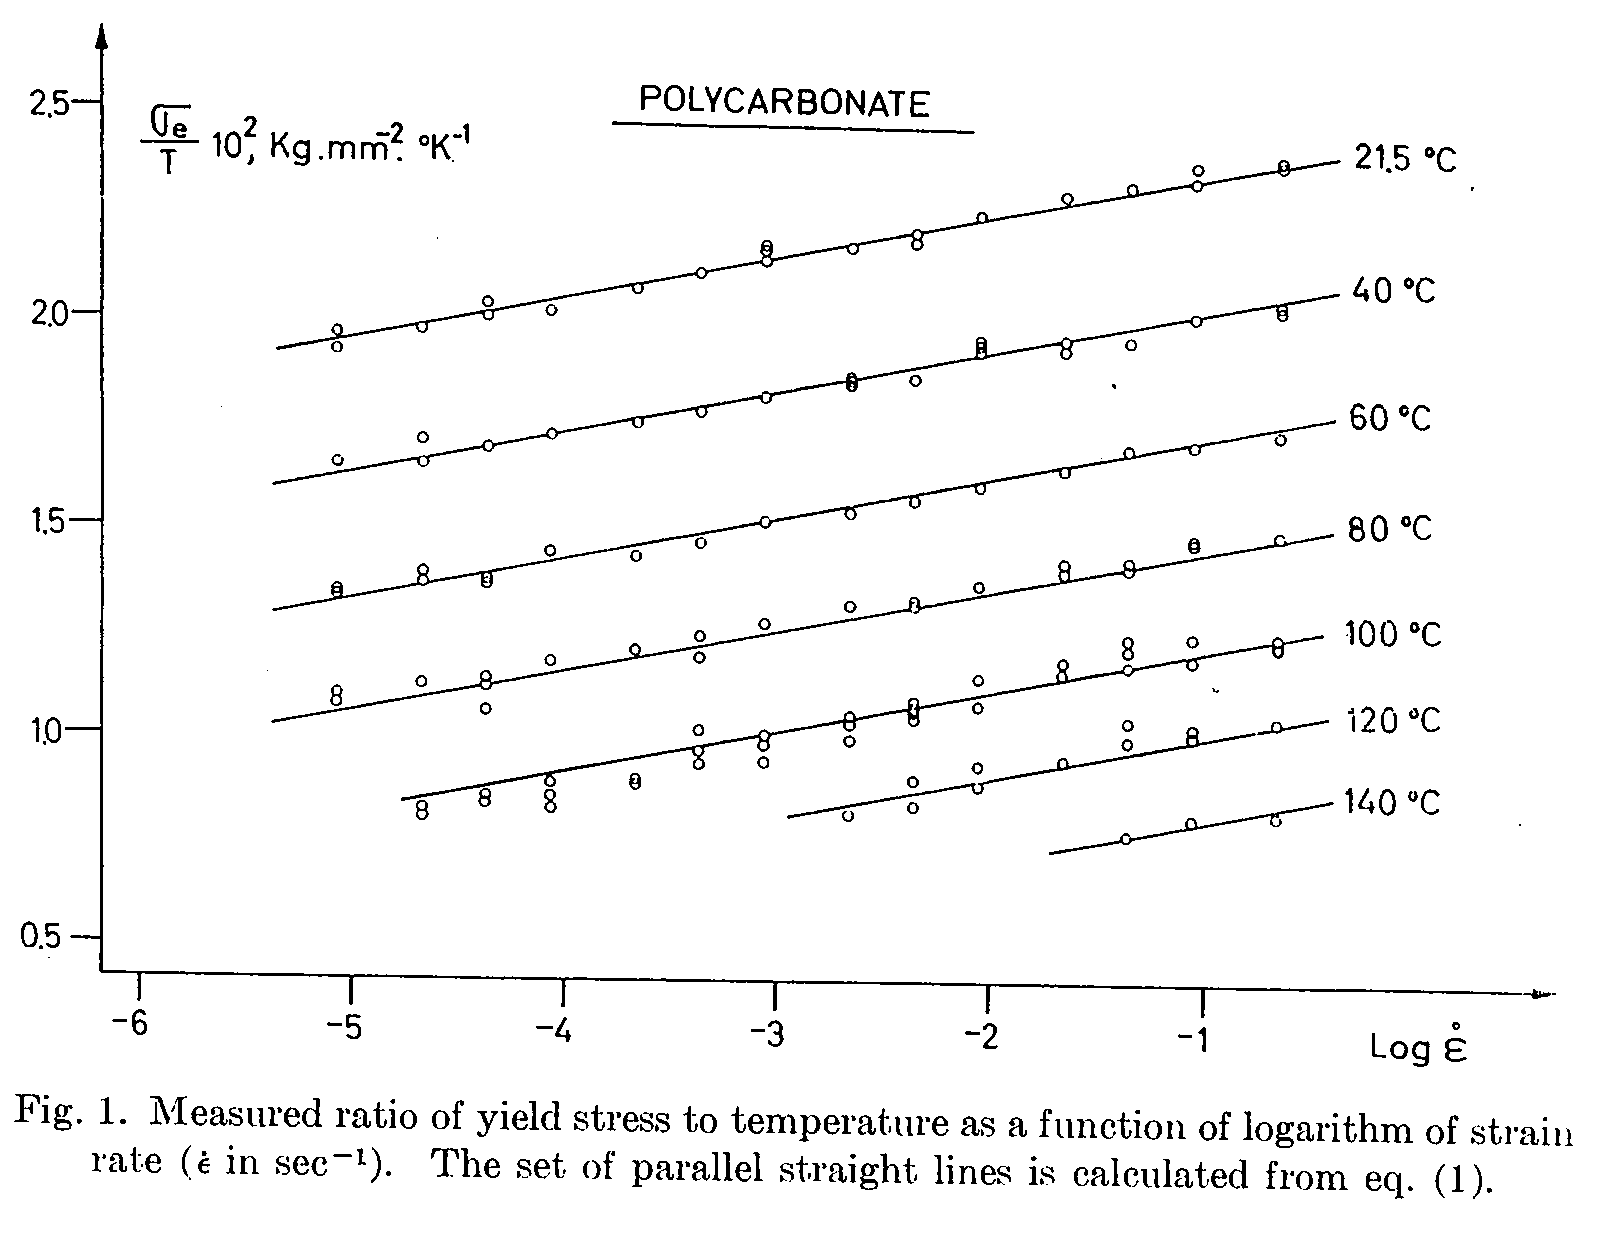
\includegraphics[width=0.5\textwidth]{fig2.png}
	\caption{PC の降伏挙動の変形速度依存性\\Copied from ref.1}
	\label{fig2}
\end{wrapfigure}

\section{背景}

PCの降伏挙動の速度依存性については過去に検討~\cite{bauwens}されており、fig.\ref{fig2} に示したような関係が報告されている。
彼らは、この片対数での線形関係は以下の表式に従っているとしている。
これは、以前に Eyring が検討したものと表式が異なっているが、この測定条件下ではこちらが妥当となるものとしている。
\begin{align}
	\dfrac{\sigma_e}{T} &= \dfrac{4\sqrt{3}k_B}{v_0 \gamma_0} \ln \left(\dfrac{\sqrt{3}}{2 \gamma_0 J_0} \dot{\epsilon} + \dfrac{Q}{RT} \right) \notag \\
	 &= A [ \ln 2 C \dot{\epsilon} + (Q/RT)]
	 \label{eq1}
\end{align}
なお、$\sigma_e$ は降伏応力(応力の最大値)、$T$ は絶対温度、$k_B$ はボルツマン因子、$v_0$ はせん断体積、$\gamma_0$ $J_0$ はエントロピー因子を含んだ速度定数、 $\dot{\epsilon}$ はひずみ速度、$Q$ は活性化エネルギーに対応する。

\newpage

\section{実験}
以下に示したように実験を行う。
\begin{description}
	\item[サンプル] 
	以下のPCサンプルを使用する
	\begin{itemize}
		\item PC2151, 0.3mm厚
		\item サンプル形状: 6 mm $\times$ 30 mm [JIS K6251 ダンベル5号の平行部を利用]
	\end{itemize}
	\item[試験条件] 
	以下の条件で測定を行う
	\begin{itemize}
		\item 温度条件
		\begin{itemize}
			\item 設定温度: 室温(一定に設定)、40, 60, 80, 100, 120\textdegree C
			\item 放置時間: チャンバー中で温度到達後30分以上放置
		\end{itemize}
		\item 試験速度
		\begin{itemize}
			\item 500, 200, 100, 50, 20, 10, 5, 2, 1, 0.5, 0.2, 0.1, 0.05, 0.02  mm/min
			\item 試験時間: 最短5秒~最大5時間
		\end{itemize}
		\item 試験終了条件
		\begin{itemize}
			\item 50mm/min以下 $\Leftrightarrow$ ストローク6mm(ε=0.2)
			\item その他 $\Leftrightarrow$ 破断検知
		\end{itemize} 
		\item 測定
		\begin{itemize}
			\item 試験力およびストロークを試験機で計測するのみ
		\end{itemize}
	\end{itemize}
	\item[データ処理] 
	測定終了後に、以下のようにデータを処理する
	\begin{itemize}
		\item 測定終了後、$\dfrac{\sigma_e}{T}$ を ヘッド速度から算出した $\dot{\epsilon}$ の対数に対してプロット
		\item \eqref{eq1} の関係から A, C, Q それぞれの値を算出する。
	\end{itemize}
\end{description}

\begin{thebibliography}{99}
    \bibitem{bauwens} C. Bauwens-Crowet, et al., J. Polym. Sci. A-2, 7(4), 735 (1969)
\end{thebibliography}

\end{document}